\section{Framework analysis}\label{sec:physical_analysis} 
In data communication and networking theory the physical layer is the lowermost
layer in the OSI model\cite{KOM}. The task of the physical layer is getting a physical signal 
translated into data which then can be delivered as a frame to the above lying layer 
which is the data link layer, all this is happening at the receiving site of the physical
layer. Communication through the physical layer would not be usable if the physical layer 
is not able to send any signal, so the physical layer would obviously have to define a set 
of tasks to translate frames from the data link layer into signals that can be transmitted. 
Thus, the physical layer defines the electrical and physical framework for receiving and 
transmitting signals through the media, and furthermore it defines encoding/decoding 
and alignment schemes for translating frames into signals and visa versa.

This project requires the use of DTMF tones as information carrier, and furthermore it is
required that transmission are broadcast through the air. These requirements decides some
of the properties of the physical layer, the first one is the media which is the air as 
sound waves are used for communication. The type of signal is DTMF tones and the communication can
only take place as half-duplex as sending and receiving is possible as the communication system works
as a broadcast system.

	\subsection{DTMF as information carrier}
	DTMF is an abbreviation for Dual Tone Multiple Frequency. It is a system of tones that are used by
	telephones when dialing a number. The system is an arrangement of four low tones and four high tones,
	it is arranged in a four-by-four matrix which gives the system sixteen combinations.
	
	The idea is that these sixteen combinations formed by the DTMF matrix is used in some kind of data
	communication between two or more computers. To let DTMF tones enter into data communication we have
	to apply the property of  waves to carry bits. This can be done by letting each entry in the matrix
	consist of four bits. Four bits gives sixteen combinations which each can be assigned to an entry in
	the matrix. Below is shown the DTMF map which will be used in the physical layer for encoding and decoding.
	
	\begin{table}[htb]
		\begin{center}
			\begin{tabular}{c|c c c c}
			 & 1209 Hz & 1336 Hz & 1477 Hz & 1633 Hz \\
			\hline
			697 Hz & 0000 & 0001 & 0010 & 0011 \\
			770 Hz & 0100 & 0101 & 0110 & 0111 \\
			852 Hz & 1000 & 1001 & 1010 & 1011 \\
			941 Hz & 1100 & 1101 & 1110 & 1111 \\
			\end{tabular}
		\end{center}
		\caption{Table of the matrix with the bit combinations assigned to each entry.}
		\label{tab:DTMF_mapping}
	\end{table}
	
	Now by letting one computer play the tones through a speaker and another computer record it from
	a microphone then data is transmitted. The exchange of data is essentially an exchange
	of information and it is not satisfying exchanging information of the size of four bits alone,
	cause this would make the system inefficient. The system need to be able to transmit a sequence
	of tones matching a given bit pattern. The number of tones played each second will determine the
	bitrate of the communication. The bitrate will of course be dependent on how fast the sampling and
	recognition of tones can be handled at the receiving end.
	
	\subsection{Port Audio Interface}
	It was decided in the initial phase of the project to use Port Audio (http://www.portaudio.com/)
	as the interface between the developed API\footnote{Application Programming Interface} and the 
	soundcard in a computer. Several points was taken into account for this decision, it has to be easy to use,
	it has access to the recorded samples and output sample buffer, and it has to be cross platform.
	Port Audio is satisfying all these needs.
	
	PortAudio is an API which exposes streams for recording or playing back sound through the soundcard of a
	computer. PortAudio allow for developers to push raw audio data to the soundcards outgoing buffer and
	receiving raw audio data from the soundcards ingoing buffer. Thus, PortAudio is good foundation for the
	implementation of the physical layer as tone detecting, and tone generating algorithms can be laid on top
	of PortAudio, as basic mathematics which apply to digital signal processing.
	
	\subsection{Goertzel Algorithm}
	To be able to detect if tones have been transmitted some algorithm for detection of tones have to be implemented.
	For this purpose the Goertzel algorithm is used, this algorithm has the ability to detect if a signal contain a
	specific frequency. Other algorithms exist which would provide the same information but those would be
	much more expensive regarding the computational complexity. Those other algorithms are called Discrete Fourier Transform (DFT)
	and the other is called Fast Fourier Transform (FFT) which is a more efficient way to obtain the same information
	as the DFT algorithm. The computational complexity of DFT\footnote{[124] Li Tan} is $N^2$, where N is the number of samples.
	For FFT\footnote{[124] Li Tan} the computational complexity is calculated to be $\frac{N}{2}\cdot log_{2}(N)$,
	where N is the number of samples.
	
	As the detection of tones has to occur as fast as possible it is desired to lower the cost of cpu power by using 
	an algorithm which has the least computational complexity. The Goertzel algorithm therefore suit this need very well.
	The reason for this is that with a few pre-calculated constants and N iterations over N samples, a value is returned
	which indicate if a specific frequency is present in the incoming signal.
	
	Essentially the Goertzel algorithm is a second order IIR filter which is dependent on current input and previous
	output, the filter is given as the difference equation shown below:
	\begin{center}\begin{equation}y(n) = x(n) + 2\cdot cos(2\pi \cdot f_{0})\cdot y(n - 1) - y(n - 2),\end{equation}\end{center}
	where $f_{0}$ is the frequency of interest.
	
	By Z-transform the following is obtained:
	\begin{center}\begin{equation}H(z) = \frac{Y(z)}{X(z)} = \frac{1}{1 - 2\cdot cos(2\pi \cdot f_{0})\cdot z^{-1} + z^{-2}}\end{equation}\end{center}
	
	As the above equation show, it is a second order IIR filter. This can be implemented as a direct form-II structure
	where the point W is of interest.
	
	\begin{figure}[htb]
		\begin{center}
		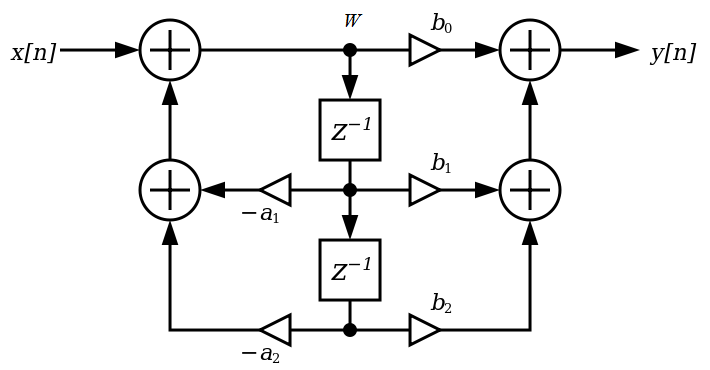
\includegraphics[scale=0.6,trim=0 0 0 0]{physical_biquad_filter.png}%trim=l b r t
		\caption{A direct form II implementation}
		\label{fig:physical_biquad_filter}
		\end{center}
	\end{figure}
	
	The point W will be used for calculating the frequency response at a specific frequency of interest. As this is taking
	place in discrete time, an expression of the frequency of interest is needed. In discrete time the frequency spectrum
	is divided into frequency bins, the size of these bins is determined by the number of samples and the sample rate.
	Obtaining the k'th bin can be done as shown below:
	\begin{center}\begin{equation}k = \frac{f_{0}}{f_{s}}\cdot N\end{equation}\end{center}
	where $f_{0}$ is the frequency of interest, $f_{s}$ is the sampling frequency, and N is the number of samples.
	
	Now it is possible to calculate the filter coefficients, which in the case with the Goertzel algorithm reduces 
	to one single coefficient. This coefficient have to be calculated for each tone that want to be identified, but can 
	be calculated in advance because its only dependent on the frequency of interest.
	
	The coefficient is calculated with:
	\begin{center}\begin{equation}c = 2\cdot cos(2\pi \cdot \frac{k}{f_{s}})\end{equation}\end{center}
	
	Now that all constants can be calculated in advance the detection system only have to calculate the filter output, calculate
	the magnitude of the frequency and then it is able to decide based on the result if the frequency exist in a incoming signal.
	As detection of DTMF tones is needed for this application it needs to determine if two specific frequencies is present at the
	same time. But this wont be much of a problem as the constants for each frequency can be calculated in advance.
	The algorithm are implemented as a direct form-II structure, and need to iterate over the array of collected samples to be
	able to detect if a given frequency is present in a signal.
	
	The computational complexity can therefore be written as one multiplication plus two additions per iteration per tone.
	This leads to:
	\begin{center}\begin{equation}numberOfOperations = 3\cdot N\cdot M,\end{equation}\end{center}
	where N is the number of samples and M is the number of tones.
	
	For one tone detection over 205 samples this is around 600 calculations, for detection of 8 tones simultaneously the equation
	above result in around 5000 calculation, and these are real calculations where as for DFT and FFT the computational complexity 
	is much higher and the calculations are carried out with complex numbers.
	
	This is the reason for choosing the Goertzel algorithm for detection of frequencies.
	
	\subsection{Synchronisation}
	The physical layer will be handling the synchronisation of the data stream. Keeping the data in sync enables the software to
	keep track of the given chunks of data from the upper layer, this is important to do because the physical layer at the receiving
	site will have to assemble the DTMF tones back into the exact same chunks of data for delivery to the upper layer.
	A way to solve this need is to wrap the content of data into a header and possibly a tail. The chuck of data received from the 
	data link layer would be natural to wrap in a header and a tail as an extra precaution to indicate if the frame is transmitted.
	This will ease the assembly of a frame because the software have an indication of the exact start of a frame and the exact ending
	of it as well.
	
	Another problem with synchronisation arise duo to the mapping between 4 bit combinations and DTMF tones. This is because if there is a
	need for sending, 1111 and 1111 right after each other the system will not be able to identify the two tones corresponding to the
	given bit patterns from each other. It would therefore look like only one tone was transmitted instead of two. This actually apply
	to each combination which are followed up by its own combination of bits. Some kind of stuffing is needed to separate each tone
	from each other.
	
	There are several ways in which this problem can be solved. One of the possibilities is to stuff the transmitted tones with a little
	bit of silence in between each other. This implementation would require some sort of timing scheme which would rely on precise timing
	so decisions, on how the recorded silence should be interpreted, can be made. Decisions that will define the transmission of a frame, will be as 
	already mentioned, where does a frame start, where does it end, and the stuffing in between each tone. All these properties will be
	hard to manage duo to silence can be considered as white noise which is totally random. White noise is not in the scope of this 
	document.
	
	A second solution could be to do the stuffing at the data link layer in between equal bit patterns with a another bit pattern. 
	The are several disadvantages duo to use of this method. First the synchronisation would now be spread across two layers because
	the physical layer still would have to track the beginning of a frame and the end of a frame. Another disadvantage is that this 
	method is unreliable as the defined bit pattern for stuffing at the data link layer could be generated by the data contained by the 
	frame itself. This mean that when data containing the bit pattern for stuffing this data could be discarded on false reasons and
	then corrupt the frame.
	
	A third and more elegant solution is to add a ninth frequency to the map seen in table \ref{tab:DTMF_mapping}. The new map will
	then look like the table below:
	
	\begin{table}[htb]
		\begin{center}
			\begin{tabular}{c c|c c c c}
	 		index & & 0 & 1 & 2 & 3 \\
			& DTMF & 1209 Hz & 1336 Hz & 1477 Hz & 1633 Hz \\
			\hline
			0 & 697 Hz & 0 & 1 & 2 & 3 \\
			1 & 770 Hz & 4 & 5 & 6 & 7 \\
			2 & 852 Hz & 8 & 9 & 10 & 11 \\
			3 & 941 Hz & 12 & 13 & 14 & 15 \\
			4 & 350 Hz & 16 & 17 & 18 & 19 \\
			\end{tabular}
		\end{center}
		\caption{This new mapping system create four new DTMF combinations, these four new DTMF tones can be used as control tones and then
		the original map as data tones. This makes it possible to identify the three properties which define the data flow in the stream.
		The index notation will be described in section \ref{sub:encoding_scheme} explains the encoding scheme.}
		\label{tab:newDTMF_mapping}
	\end{table}
		
	\subsection{Encoding scheme}\label{sub:encoding_scheme}
	Jubii
